\pdfoutput=1
\documentclass{article}
\usepackage[utf8]{inputenc}
\usepackage[review]{acl}
\usepackage{times}
\usepackage{latexsym}
\usepackage{graphicx}
\usepackage{authblk}
\usepackage[T1]{fontenc}
\usepackage[utf8]{inputenc}
\usepackage{microtype}
\usepackage{amsmath}


\title{AbuseBert - BERT language model to detect Abuse sentences}


\author{Balakrishna A, \\
  Undergraduate Bachelor of Technology, \\
  Computer Science and Engineering, \\
  Vishnu Institute of technology, \\
  Bhimavaram,  \\
  Andhra Pradesh, \\
  India, \\
  \texttt{baluakula2000@gmail.com} \\}
\date{Sepetember 30 2022

\begin{document}
\maketitle{}
\begin{abstract}
This paper describes the experimentation on how the BERT model is used to predict the Abusive content in a given text. It was found that the model is working on to the most of the extent. This paper addresses the solution to the detection of Abusive content by taking BERT into consideration. There are other approaches done by researches by customizing attention probabilities and boosting based with BERT models. However, this paper shows the output layer that was introduced to distinguish and modification of the masking to particular contextual words that are actually abuse with the backbone of Abuse contextualised language model. The model achieves 75-80\% 
accuracy on most of the Abusive text. The progression of this work is extended to pass deep contextualised word embeddings by ELMo using biLMs for to Abuse contextualised language model. 
\end{abstract}

\section{Introduction}
In many platforms on social media, Abusive detection is the prominent role to set users in discipline. Despite prevailing models, it is still needed to find the multilingual Abusive text detection models. The study of the BERT\cite{vaswani2017attention} transformer puts its own way of strong foundation on the language model which developers modifies, fine-tune for their sake of work(specifically for Abusivhateoffensivee detection). Some of the previous works are Gradient Boosting along with BERT and LASER embeddings, XGboost, LGBM, m-BERT models trained on Hindi, Urdu, English languages. But, most of the researches found that BERT performance is far better than any other models to detect.

Detection of abusive language in online can view as a union of the plethora of
subtasks that had been faced such as sexism, Harassment with sentiment words, Hate Speech, racism, trolling, etc. Now this is particularly focusing on subtasks of language model to learn some of kind of intuition about Abuse context. Several arguments such as\cite{schmidt-wiegand-2017-survey} reveals that due to this phenomenon
where works restricted subsets of abusive language, it will become difficult to make justifications about whether the features being used can
perform well in other subtasks of abusive language
detection.

In this model, at the bottom, it has a contextualised language model that is used to predict the Hate or Non-Hate  by applying output layer. In the output layer, the model consists of Batch-Normalization is used to normalize the BERT output embedding followed by two linear layers introduced with ReLU activation function. Softmax with two labels is applied on the output to distinguish the sentence is actually abusive or not. The second work in this model is masking was applied to the keywords that are typically abusive before sending the masked sentence to the decode layer. Therefore, the model has a contextualised language model\cite{kutuzov2021large} that aims for able to learn the distinction between Hate or Non-Hate. We then maps this language model to our labels as Abuse or No-Abuse at the output layer.

Currently, from the recent papers, the concept of deep contextualised word embedding improves the state-of-the-art of the transformer model. Considering this concept, the working progress is going on to achieve good accuracy for the model to detect the Hate contextualised sentence.

\section{Related Work}
Abusive language Detection in the field of Natural Language Processing has recently scored good attraction
among the researchers. However, the task of detecting technologies is still going by several researchers through language models to process natural languages.In 2017, Waseem et al.\cite{waseem-etal-2017-understanding} classify abusive languages into two category “Directed" which is the
language directed towards a specific individual or entity and “Generalized" (directed towards a generalized group), further this category divided into another two category “Explicit"
and “Implicit" (the degree to which it is explicit).


Davidson et al\citep{hateoffensive} collected a dataset that comprises of thousands of tweets which are labeled as "hate", "offensive", and "neither", with the classification task of detecting hate/offensive speech present
in Tweets. They explored how linguistic features such as  word n-grams character and affects the performance of a classifier that aims to distinguish the tweets that labels as "hate", "offensive", and "neither". Additional features in their classification involved binary and count
indicators for hashtags, mentions, retweets, and URLs, as well as features for the number of
characters, words, and syllables in each tweet. The issues found by the researches with this model, is not distingushing the hate and offensive posts.
In 2018, Karan and Snajder\cite{karan-snajder-2018-cross} experimented with
cross-domain training and testing, They choosed to use
the model (LSVM) with minimal features
and to preprocess in favour of interpretability.
They also reported positive improvements using
Frustratingly Easy Domain Adaptation\cite{DBLP:journals/corr/abs-0907-1815} to augment smaller datasets with
larger ones. It was discussed that although model is obtaining good performance statistically, It has to be trained on huge train data to worth the model predicting level.

Similarly, Waseem
et al, in 2018\cite{elsherief2021latent},builds a robust
multi-task learning model addresses the problem of
differences between datasets, which improves on
single-task performance by using auxiliary sam-
ples from select datasets. It was revealed that their work on such models could be competitive with the state-
of-the-art single-task models with the additional
benefit of allowing prediction on other datasets as
well. This helps in promoting generalisability and negating hidden biases within datasets.

In 2019, Hate-Monitors, Language Agnostic abuse Detection in social media\cite{DBLP:journals/corr/abs-1909-12642} used the Gradient Boosting along with BERT and LASER embeddings to make language model agnostics. They have done on three different languages. Except to German sentences, the model got good accuracy on English and hindi. 

Recently, In 2021, Abusive and Threatening Language Detection in
Urdu using Boosting based and BERT based models\cite{DBLP:journals/corr/abs-2111-14830} cameup with a Comparative Approach that
they have attempted several models for abusive and threatening detection task. As a baseline they tried XGBoost and LightGBM with pretrained Urdu
laser embedding. Later they have tried Transformer-based pre-trained architecture of multilingual
BERT.The beauty of the mBERT is it is pretrained in unsupervised manner on multilingual

\section{Analysis}
Several previous works in online Abuse language detection focused on solving a single abusive language problem in a single domain, like Twitter, and have not been successfully transferable to the general Abuse language detection task or domain. 

The latest publication paper of Abusive and Threatening Language Detection in Urdu using Boosting based and BERT based models giving excellent score, but the model is trained on Native Languages. 

Another model 'Detect All Abuse! Toward Universal Abusive Language Detection Models'\cite{wang-etal-2020-detect}, provides results on three random samples of our dataset as follows,
\begin{table}[h]
\begin{tabular}{llll}
\hline
Sample & Precison & Accuracy & Recall \\
\hline 
1.  &0.76     & 0.50     & 0.61   \\
2.  &0.49     & 0.75     & 0.59   \\
3.  &0.60     & 0.60     & 0.60  
\end{tabular}

\caption{Results of the model on three custom records}
\label{tab:accents}
\end{table}
These results shows that it still needs a good model, specifically speaking about good abuse contextualised model. The analysis of requiring the best language model leads to use make BERT model that can specifically distinguishes Hate or Non Hate .

\section{Design}
In the design phase, using BERT model, the sentences are masked to particular words with the keywords that are actually abuse. Secondly, the output layer is designed to sigmoid the two labels as Abuse or no-Abuse. 

In the first step, we tokenize the sentence, and segregate the Abuse context words by using the List of Hate words. Every time we map whether the word in the sentence is in our bag of Abuse words. Next, The model will get trained to learn a language model to identify the Abuse contextualisation by predicting those masked words at the Multi head attention\cite{choi2018fine} sublayer in the decode layer.

\begin{figure}[h]
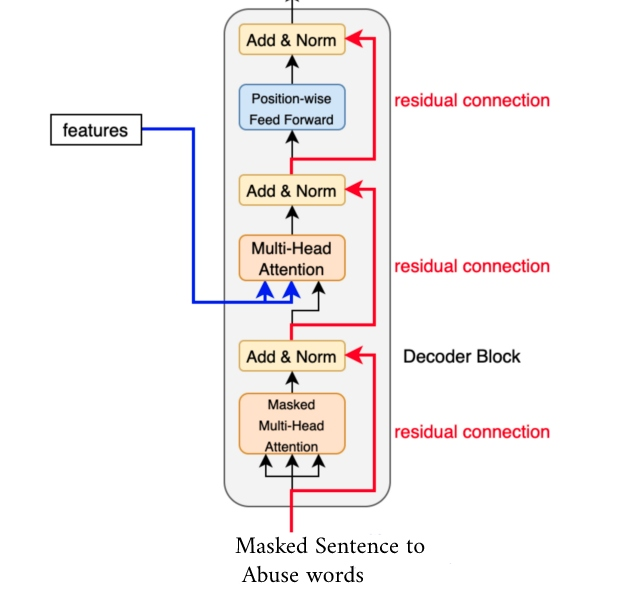
\includegraphics[width=8cm]{images/Myopic.jpg}
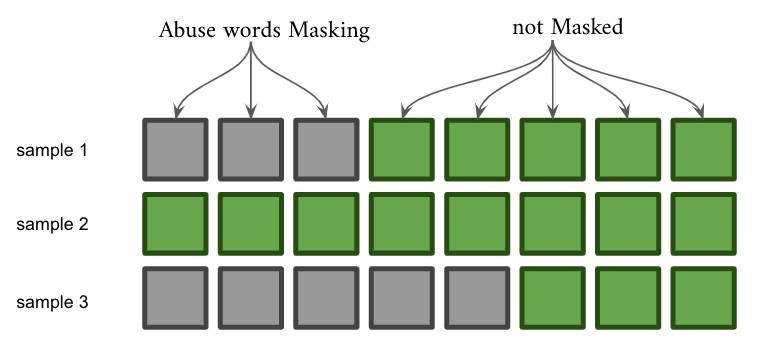
\includegraphics[width=8cm]{images/attention_mask.jpg}

\caption{ This figures demonstrate the Abuse words masking and pipe-lining this masked sentence to the next sublayer Multi-Head Attention }
\label{fig:AttentionFig}
\end{figure} 

Further, The language model contextualisation can also be increased by introducing ELMo\cite{peters-etal-2018-deep} from the paper Deep contextualized word representations.
Although Attention is applied to the tokens, We still pass the contextualised tokens instead of tokens to the BERT model that can efficiently utilizes the ELMo embeddings. this token can be used as contextualisation token.
Basically ELMo embeddings for the particular task of kth token can be shown as,
\begin{equation*}
    \mathrm{ELMo}_{k}^{Hatetask} = E(\mathrm{R}_{k}^{};\mathrm{\Theta}^{Hatetask}) = \mathrm{\gamma}^{task}\sum_{j=0}^{L}\mathrm{s}_{j}^{Hatetask}\mathrm{h}_{k,j}^{LM}
\label{adkfdfi}
\end{equation*} 

Here, $\mathrm{x}_{j}^{LM}$ is the contextualised token that was generated via token embeddings or a CNN over characters. It is the representation of the jth token to the for the biLM\cite{amrami2018word}. This $\mathrm{x}_{j}^{LM}$ is passed to the biLM(bidirectional Language model). The $\mathrm{h}_{k,j}^{LM}$ in the equation is the obtained token at the each layer in biLMs. ELMo takes all of these sums with applying $\gamma^{task}$ and $\mathrm{s}_{k}^{task}$ parameters. We can also go through this approach. This approach tends to pass contextulaised tokens instead of BERT tokens by the BERT tokenizer. The significance od this approach is the model can learn more Abuse sentence specific language models. In this paper, we have only implemented up to the masking of specific words in the given sentence to learn abuse contextualised language model.

For the output layer, The Batch Normalization\cite{bjorck2018understanding} applied to the output of the BERT embeddings. These are passed to the two linear layers with ReLU activation function in the both layers. The output is obtained by soft-maxing(with number of labels = 2) the last linear+ReLu layer.

\begin{figure}[h]
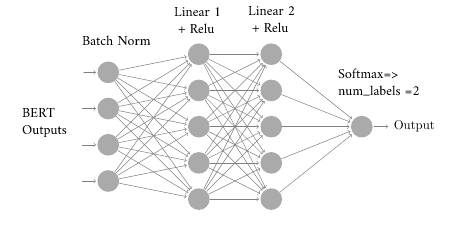
\includegraphics[width=8cm]{images/OutputlayerMod.jpg}
\caption{}
\label{fig:AttentionFig}
\end{figure}

% The first line of the file must be
% \begin{quote}
% \begin{verbatim}
% \documentclass[11pt]{article}
% \end{verbatim}
% \end{quote}
\section{Development \& Implementation}
As a new research content(experimented), we found to build a language model on Abuse word  context. About the dataset, it was collected from different online resources. Some of are, Wikipedia, HateBase.org ,T.Davidson GitHub.

\begin{table}[h]
\vline\vline
\begin{tabular}{|l|l|}
\hline
Post Text                                   & Hate/No-Hate \\ \hline
Want to HateF*ck Date? Sure.                & 2.0          \\ 
Sounds good now I am hungry LOL             & 1.0          \\ 
Memes are what gets me every time.          & 1.0          \\ 
Shint cunt. Civnat faggotry is for faggots. & 2.0          \\ 
What a screaming load of shit!              & 1.0          \\ 
\hline
\end{tabular}
\caption{Dataset example view}
\end{table}

To collect this data set, we use selenium web scratch technologies to extract more abuse sentences and direct download options in the websites itself. Most of this data set used Hate-base.org. The labels are floating point numbers 1.0,2.0 indicating No-Hate, Hate. 

\begin{table}[]
\vline\vline
\begin{tabular}{|l|l|}
\hline
Total train data & 6400             \\ \hline
Total test data  & 1600             \\ \hline
Total epochs     & 14.0             \\ \hline
Batch size       & 5.0              \\ \hline
Loss function    & Cross Entropy    \\ \hline
Optimizer        & Adam Optimizer   \\ \hline
Scheduler        & Cosine Annealing \\ \hline
\end{tabular}
\caption{Training details}
\end{table}\\

There are totally 8000 records in the data set. The train test split ratio for this data set is 0.95:0.5 and it is trained on 14 epochs with batch size 5.

We use BERT(base uncased) model to train the language model from hugging face. PyTorch, transformers, and other utilities are used in the code.
\section{Evaluation}

In the testing phase, we evaluate the model on how it is working with different real world abuse sentences.  We have total 1600 records of test data-set. The results are shown below.
\begin{figure}[h]
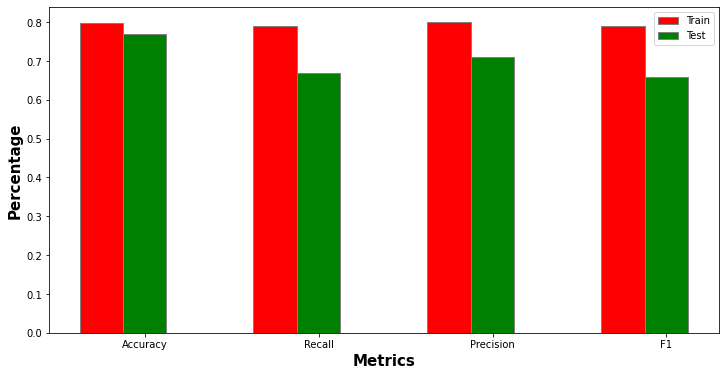
\includegraphics[width=8cm]{images/download.png}
\caption{Train and test metrics}
\label{fig:GraphFig}
\end{figure}
\begin{table}[h]
\vline\vline
\begin{tabular}{|l|l|l|l|l|}
\hline
      & Accuracy & Precision & Recall & F1   \\ \hline
TRAIN & 0.798    & 0.79      & 0.80   & 0.79 \\ \hline
TEST  & 0.77     & 0.67      & 0.71   & 0.66 \\ \hline
\end{tabular}
\caption{Table of Train and test metrics}
\end{table}

\section{Conclusion}
This approach significantly predicts the sentences having Abuse meaning relations. But the drawback here is, that we need to specify the masking on abuse words. So we have to require the bag of Hate words. One may also think that, why not we iterate the sentence and make a decision whether it is abuse or not by simply mapping abuse words in the sentence to bag of abuse words. But, the situation here is, we are trying to maintain a meaning to the entire sentence from the language model. For instance, Pussy, Pussycat are entirely different. This meaning reflects along with entire sentence and thus able to make sense of predicting a sentence as Abuse or not by using the language model.

The deep contextualised embedding tokens can also apply on the task specific(BERT, output) models. These embedding contains the relation between different words and thus able to accurate the deep Abuse language model. However, In this paper it was experimented up to to the masking specific words and creating out put layer tat distinguishes the Hate or Non Hate.

\bibliography{custom}
\bibliographystyle{acl_natbib}


% \begin{thebibliography}{9}
\bibitem{vaswani2017attention}
Vaswani, Ashish, \emph{Attention is all you need}, Advances in neural information processing systems, 2017.

\bibitem{schmidt-wiegand-2017-survey}
Schmidt, Anna  and \emph{Wiegand, Michael", Proceedings of the Fifth International Workshop on Natural Language Processing for Social Media}, 2017.

\bibitem{kutuzov2021large}kutuzov2021large
Kutuzov, Andrey and Barnes, \emph{Large-scale contextualised language modelling}, 2021.

\bibitem{waseem-etal-2017-understanding}
Waseem, Zeerak  and Davidson, \emph{Understanding Abuse: A Typology of Abusive Language Detection Subtasks}, 2017.

\bibitem{hateoffensive}
Davidson, Thomas and Warmsley, \emph{Automated Hate Speech Detection and the Problem of Offensive Language}, 2017.

\bibitem{karan-snajder-2018-cross}
Karan, Mladen  and najder, \emph{Cross-Domain Detection of Abusive Language Online}, 2018.

\bibitem{DBLP:journals/corr/abs-0907-1815}
Hal Daum, \emph{Frustratingly Easy Domain Adaptation}, 2009.

\bibitem{elsherief2021latent}
ElSherief, Mai and Ziems Implemented Waseem et al. addresses, \emph{Latent hatred: A benchmark for understanding implicit hate speech}, 2021.

\bibitem{DBLP:journals/corr/abs-1909-12642}
Punyajoy Saha and Binny Mathew, \emph{HateMonitors: Language Agnostic Abuse Detection in Social Media}, 2019.

\bibitem{DBLP:journals/corr/abs-2111-14830}
Mithun Das and Somnath Banerjee, Abusive and Threatening Language Detection in Urdu using Boosting based and {BERT} based models:{A} Comparative Approach, 2021.

\bibitem{wang-etal-2020-detect}
Wang, Kunze  and Lu, Dong\emph{Detect All Abuse! Toward Universal Abusive Language Detection Models}, 2020.

\bibitem{choi2018fine}
Choi, Heeyoul and Cho \emph{attention mechanism for neural machine translation}, 2018.

\bibitem{peters-etal-2018-deep}
Peters, Matthew E, \emph{Deep Contextualized Word Representations}, 2018.

\bibitem{bjorck2018understanding}
Bjorck, Nils and Gomes, \emph{Understanding batch normalization}, 2018.

\bibitem{amrami2018word}
amrami2018word, \emph{Word sense induction with neural biLM and symmetric patterns}, 2018.










% \end{thebibliography}
% \section{Example Appendix}
% \label{sec:appendix}

\end{document}
